\chapter{Constructing New Vector Bundles Out of Old}

This section will describe a number of basic constructions involving
vector bundles.

\subsection*{Restricting a bundle to a subset of the base space} Let $\xi$ be a
	vector bundle with projection $\pi\mathpunct{:} E\to \B$ and let $\bar{\B}$ be a subset of $\B$.
	Setting $\bar{E}=\pi\inv(\bar{\B})$, and letting
	\[\bar{\pi}\mathpunct{:}\bar{E}\longrightarrow \bar{\B} \]
	be the restriction of $\pi$ to $\bar{E}$, one obtains a new vector bundle which
	will be denoted by $\xi|_{\bar{\B}}$, and call the \textit{restriction} of $\xi$ to $\bar{\B}$. Each
	fiber $F_b(\xi|_{\bar{\B}})$ is equal to the corresponding fiber $F_b(\xi)$, and is to be
	given the same vector space structure.
	
	As an example if $M$ is a smooth manifold and $U$ is an open subset
	of $M$, then the tangent bundle $\tau_U$ is equal to $\tau_M|_{U}$.

More generally one has the following construction.


\subsection*{Induced bundles} Let $\xi$ be as above and let $\B_1$ be an arbitrary
	topological space. Given any map $f\mathpunct{:} \B_1\to \B$ one can construct the 
	induced bundle $f^*\xi$ over $\B_1$. The total space $E_1$ of $f^*\xi$ is the subset
	$E_1 \subset \B_1 \times E$ consisting of all pairs $(b, e)$ with
	$f(b)=\pi(e)$. The projection map $\pi_1\mathpunct{:}E_1\to \B_1$ is defined by $\pi_1(b,e)=b$. Thus one
	has a commutative diagram
\[\begin{tikzcd}
		E_1 \arrow[r, "\hat{f}"] \arrow[d, "\pi_1", swap] &E \arrow["\pi", d] \\
		\B_1 \arrow[r, "f"]           & \B          
\end{tikzcd}\]
where $\hat{f}(b, e) = e$. The vector space structure in $\pi\inv(b)$ is defined by
\[t_{1}\left(b, e_{1}\right)+t_{2}\left(b, e_{2}\right)=\left(b, t_{1} e_{1}+t_{2} e_{2}\right). \]
Thus $\hat{f}$ carries each vector space $F_b(f^*\xi)$ isomorphically onto the 
vector space $F_{f(b)}(\xi)$.

If $(U,h)$ is a local coordinate system for $\xi$, set $U_1 = f\inv(U)$ and
define
\[h_{1}\mathpunct{:} U_{1} \times \R^{n} \longrightarrow \pi_{1}^{-1}\left(U_{1}\right),\]
by $h_{1}(b, x)=(b, h(f(b), x))$. Then $(U_1, h_1)$ is clearly a local coordinate
system for $f^*\xi$. This proves that $f^*\xi$ is locally trivial. (If $\xi$ happens
to be trivial, it follows that $f^*\xi$ is trivial.)

\begin{remark*}
	If $\xi$ is a smooth vector bundle and $f$ a smooth map, then
	it can be shown that $E_1$ is a smooth submanifold of $\B_1 \times E$, and hence
	that $f^*\xi$ is also a smooth vector bundle.
\end{remark*}

The above commutative diagram suggests the following concept which
a priori, is more general. Let $\xi$ and $\eta$ be vector bundles.

\begin{definition}\label{def:3-1}
	A \textit{bundle map} from $\eta$ to $\xi$ is a continuous function
	\[g\mathpunct{:}E(\eta)\longrightarrow E(\xi), \]
	which carries each vector space $F_b(\eta)$ isomorphically onto one of the
	vector spaces $F_{b'}(\xi)$.
\end{definition}

Setting $\bar{g}(b) =
b'$, it is clear that the resulting function
\[\bar{g}\mathpunct{:}\B(\eta)\longrightarrow \B(\xi), \]
is continuous.

\begin{lemma}\label{lem-3-1}
	If $g\mathpunct{:}E(\eta)\rightarrow E(\xi)$ is a bundle map, and if
	$\bar{g}\mathpunct{:}\B(\eta)\rightarrow \B(\xi)$  is the corresponding map of base spaces, then
	$\eta$ is isomorphic to the induced bundle $\bar{g}^*\xi$.
\end{lemma}

\begin{proof}
	Define $h\mathpunct{:}E(\eta)\rightarrow E(\bar{g}^*\xi)$ by $h(e)=(\pi(e),g(e))$ where $\pi$ denotes the projection map of $\eta$. Since $h$ is continuous and
	maps each fiber $F_b(\eta)$ isomorphically onto the corresponding fiber
	$F_b(\bar{g}^*\xi)$, it follows from \cref{lem-2-3} that $h$ is an isomorphism.
\end{proof}
\subsection*{Cartesian products}
Given two vector bundles $\xi_1$, $\xi_2$ Projection maps $\pi_i\mathpunct{:}E_i\to \B_i$, $i =
1, 2$, the \textit{Cartesian product}  $\xi_1\times\xi_2$ is defined to be the bundle with projection map
\[\pi_1\times\pi_2\mathpunct{:}E_1\times E_2\longrightarrow \B_1\times\B_2;\]
where each fiber
\[\left(\pi_{1} \times \pi_{2}\right)^{-1}\left(b_{1}, b_{2}\right)=F_{b_{1}}\left(\xi_{1}\right) \times F_{b_{2}}\left(\xi_{2}\right), \]
is given the obvious vector space structure. Clearly $\xi_1\times\xi_2$ is locally
trivial.


As an example, if $M = M_1 \times M_2$ is a product of smooth manifolds,
then the tangent bundle $\tau_M$ is isomorphic to $\tau_{M_1}\times \tau_{M_2}$
(Compare
\cref{prob-1-A}.)
\subsection*{Whitney sums}
Next consider two bundles $\xi_1$, $\xi_2$ over the same
base space $\B$. Let
\[d\mathpunct{:}\B\longrightarrow \B\times\B \]
denote the diagonal embedding. The bundle $d^*(\xi_1\times\xi_2)$ over $\B$ is
called the \textit{Whitney sum} of $\xi_1$ and $\xi_2$; and will denoted by $\xi_1\oplus\xi_2$.
Note that each fiber $F_b(\xi_1\oplus\xi_2)$ is canonically isomorphic to the direct
sum
$F_b(\xi_1)\oplus F_b(\xi_2)$.
\begin{definition}\label{def:3-2}
	Consider two vector bundles $\xi$ and $\eta$ over the same base space $\B$ with $E(\xi ) \subset E(\eta)$; then $\xi$ is a \textit{sub-bundle} of $\eta$ (written
	$\xi\subset\eta$) if each fiber $F_b(\xi)$ is a sub-vector space of the corresponding fiber $F_b(\eta)$.
\end{definition}
\begin{lemma}\label{lem-3-2}
	Let $\xi_1$ and $\xi_2$ be sub-bundles of $\eta$ such that
	each vector space $F_b (\eta)$ is equal to the direct sum of the sub-spaces $F_b (\xi_1)$ and $F_b (\xi_2)$. Then $\eta$ is isomorphic to the
	Whitney sum $\xi_1\oplus\xi_2$.
\end{lemma}
\begin{proof}
	Define $f\mathpunct{:}E(\xi_1\oplus\xi_2)\to E(\eta)$ by $f(b,e_1,e_2) =
	e_1 + e_2$. It 
	follows from \cref{lem-2-3} that $f$ is an isomorphism.
\end{proof}
\subsection*{Orthogonal complements}
This suggests the following question.
Given a sub-bundle $\xi\subset\eta$ does there exist a complementary sub-bundle
so that $\eta$ splits as a Whitney sum? If $\eta$ is provided with a Euclidean
metric then such a complementary summand can be constructed as follows.\footnote{If the base space $\B$ is paracompact then $\eta$ can always be given a Euclidean
	metric (\cref{prob-2-C}); hence a sub-bundle $\xi\subset\eta$ is always a Whitney summand. If
	$\B$ is not required to be paracompact, then counterexamples can be given.}

Let $F_b(\xi^\perp)$ denote the subspace of $F_b(\eta)$ consisting of all vectors
$v$ such that $v \bdotp
w = 0$ for all $w\in
F_b(\xi)$. Let $E(\xi^\perp) \subset E(\eta)$ denote the
union of the $F_b(\xi^\perp)$.


\begin{definition}\label{def:3-3}
	$\xi^\perp$ will be called the orthogonal complement of $\xi$ in $\eta$.
\end{definition}

\begin{theorem}\label{thm-3-3}
	$E(\xi^\perp)$ is the total space of a sub-bundle
	$\xi^\perp\subset\eta$. Furthermore $\eta$ is isomorphic to the Whitney sum $\xi_1\oplus\xi_2$.
\end{theorem}
\begin{proof}
	Clearly each vector space $F_b(\eta)$ is the direct sum of the sub-spaces $F_b(\xi)$ and $F_b(\xi^\perp)$. Thus the only problem is to prove that $\xi^\perp$
	satisfies the local triviality condition.
	
	Given any point $b_0\in \B$, let $U$ be a neighborhood of $b_0$ which is
	sufficiently small that both $\xi|_U$ and $\eta|_U$ are trivial. Let $\coord{s_m}$
	be normal orthogonal cross-sections of $\xi|_U$ and let $\coord{{s'}_n}$ be
	normal orthogonal cross-sections of $\eta|_U$; where $m$ and $n$ are the 
	respective fiber dimensions. (Compare \cref{lem-2-4}.) Thus the $m\times n$ matrix 
	\[\left[s_{i}\left(b_{0}\right) \bdotp s_{j}^{\prime}\left(b_{0}\right)\right], \]
	has rank $m$. Renumbering the $s'_j$ if necessary, we may assume that the
	first $m$ columns are linearly independent.
	
	Let $V\subset U$ be the open set consisting of all points $b$ for which the
	first $m$ columns of the matrix $[s_{i}(b) \bdotp s_{j}^{\prime}(b)]$  are linearly independent.
	Then the $n$ cross-sections
	\[\coord{s_m},s'_{m+1},\dots,s'_n \] 
	of $\eta|_U$ are not linearly dependent at any point of $V$. (For a linear 
	relation would imply that some non-zero linear combination of $\coord{s_mb}$
	was also a linear combination of $s'_{m+1}(b),\dots,s'_n(b)$, hence orthogonal to
	$\coord{{s'}_mb}$.) Applying the Gram-Schmidt process to this sequence of
	cross-sections, we obtain normal orthogonal cross-sections $\coord{s_m},$ $s_{m+1},\dots,s_n$ of $\eta|_V$.
	
	Now a local coordinate system
	\[h\mathpunct{:}V\times\R^{n-m}\longrightarrow E(\xi^\perp), \]
	for $\xi^\perp$ is given by the formula
	\[h(b, x)=x_{1} s_{m+1}(b)+\cdots+x_{n-m} s_{n}(b).\]
	The identity
	\[h^{-1}(e)=\left(\pi e,\left(e \bdotp s_{m+1}(\pi e), \ldots, e \bdotp s_{n}(\pi e)\right)\right),\]
shows that $h$ is a homeomorphism, and completes the proof of \ref{thm-3-3}.
\end{proof}

As an example, suppose that $M\subset N\subset \R^A$ are smooth manifolds, and
suppose that $N$ is provided with a Riemannian metric. Then the tangent
bundle $\tau_M$ is a sub-bundle of the restriction $\tau_N|_M$. In this case the
orthogonal complement $\tau_M^\perp\subset\tau_N|_M$ is called the \textit{normal bundle} $\nu$ of $M$
in $N$. Thus we have:

\begin{corollary}
	For any smooth submanifold $M$ of a smooth
	Riemannian manifold $N$ the normal bundle $\nu$ is defined, and
	\[\tau_M\oplus\nu\subset\tau_N|_M. \]
\end{corollary}


More generally a smooth map $f \mathpunct{:} M \to N$ between smooth manifolds is
called an immersion if the Jacobian
\[\mathsf{D}f_x\mathpunct{:} \mathsf{D}M_x\longrightarrow \mathsf{D}Nf_{(x)}\]
maps the tangent space $\mathsf{D}M_x$ injectively (i.e., with kernel zero) for each
$x\in M$. [It follows from the implicit function theorem that an immersion is
locally an embedding of $M$ in $N$, but in the large there may be self-intersections. A typical immersion of the circle in the plane is illustrated in \cref{fig4}.]

\begin{figure}[!htb]
	\centering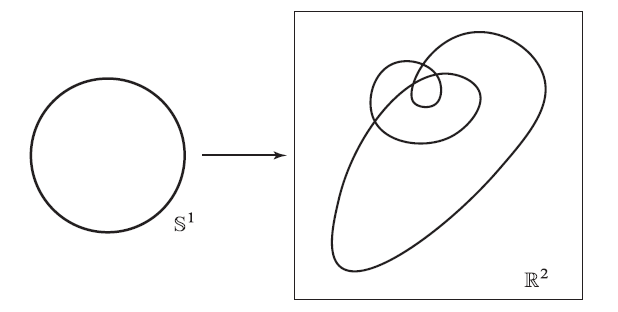
\includegraphics[scale=.6]{fig4}
	\caption{}\label{fig4}
\end{figure}

Suppose that $N$ is a Riemannian manifold. Then for each $x\in M$, the
tangent space $\mathsf{D}N_{f(x)}$ splits as the direct sum of the image $\mathsf{D}f_x(\mathsf{D}M_x)$
and its orthogonal complement. Correspondingly the induced bundle $f^*\tau_N$
over $M$ splits as the Whitney sum of a sub-bundle isomorphic to $\tau_M$ and
a complementary sub-bundle $\nu_f$. Thus:

\begin{corollary}\label{cor-3-5}
	For any immersion $f \mathpunct{:} M\to
	N$, with $N$
	Riemannian, there is a Whitney sum decomposition
	\[f^*\tau_N\cong \tau_M\oplus\nu_f.\]
\end{corollary}
This bundle $\nu_f$ will be called the \textit{normal bundle} of the immersion $f$.

\subsection*{Continuous functors of vector spaces and vector bundles}
The
direct sum operation is perhaps the most important method for building
new vector spaces out of old, but many other such constructions play an
important role in differential geometry. For example, to any pair $V, W$ of
real vector spaces one can assign:

\begin{enumerate}[label=\arabic*),leftmargin=2\parindent ]
	\item the vector space $\hom(V, W)$ of linear transformations from $V$ to
	$W$;
	\item the tensor product\footnote{See for example \cite[pp. 408, 424]{3}.} $V\otimes W$;
	\item the vector space of all symmetric bilinear transformations from
	$V \times V$ to $W$; and so on.
\end{enumerate}
To a single vector space $V$ one can assign:

\begin{enumerate}[resume,label=\arabic*),leftmargin=2\parindent ]
	\item the dual vector space $\hom(V, \R)$;%\setcounter{footnote}{1}
	\item the $k$-th exterior power\footnote{See for example \cite[pp. 408, 424]{3}.} $\Lambda^k V$;
	\item the vector space of all $4$-linear transformations
	$V \times V\times V \times V\to \R$ satisfying the symmetry relations:
	\[ K(v_1,v_2,v_3,v_4)=K(v_3,v_4,v_1,v_2)=-K(v_1,v_2,v_4,v_3)\]
	and
	\[ K(v_1,v_2,v_3,v_4)+K(v_1,v_4,v_2,v_3)+K(v_1,v_3,v_4,v_2)=0.\]
\end{enumerate}
(This last example would be rather far-fetched, were it not important in
the theory of Riemannian curvature.)

These examples suggest that we consider a general functor of several vector space variables.

\begin{definition}\label{def:3-4}
	Let $\mathcal{O}$ denote the category consisting of all finite dimensional real
	vector spaces and all isomorphisms between such vector spaces. By a
	(covariant\footnote{The distinction between covariant and contravariant functors is not important
		here, since we are working only with isomorphisms.}) \textit{functor} $T \mathpunct{:} \mathcal{O}\times\mathcal{O} \to \mathcal{O}$ is meant an operation which assigns
	\begin{enumerate}[label=\arabic*),leftmargin=2\parindent ]
		\item to each pair $V, W\in \mathcal{O}$ of vector spaces a vector space $T(V, W)\in\mathcal{O}$;
	\end{enumerate}
	and
	\begin{enumerate}[label=\arabic*),leftmargin=2\parindent,resume ]
		\item to each pair $f\mathpunct{:} V \to V'$, $g \mathpunct{:} W \to W'$ of isomorphisms an isomorphism
		\[T(f, g): T(V, W) \rightarrow T\left(V^{\prime}, W^{\prime}\right);\]
	\end{enumerate}
	so that
	\begin{enumerate}[label=\arabic*),leftmargin=2\parindent,resume ]
		\item $T(\id_V,\id_W)=\id_{T(V,W)}$ and
		\item $T\left(f_{1} \circ f_{2}, g_{1} \circ g_{2}\right)=T\left(f_{1}, g_{1}\right) \circ T\left(f_{2}, g_{2}\right)$.
	\end{enumerate}
Such a functor will be called \textit{continuous} if $T(f, g)$ depends continuously
on $f$ and $g$. This makes sense, since the set of all isomorphisms from
one finite dimensional vector space to another has a natural topology.
\end{definition}

The concept of a continuous functor $T\mathpunct{:}\mathcal{O}\times\dots\times\mathcal{O}\to\mathcal{O}$ in $k$ variables
is defined similarly. Note that examples 1, 2, 3 above are continuous
functors of two variables, and that examples 4, 5, 6 are continuous 
functors of one variable.

Let $T\mathpunct{:}\mathcal{O}\times\dots\times\mathcal{O}\to\mathcal{O}$ be such a continuous functor of $k$ variables,
and let $\coord{\xi_k}$ be vector bundles over a common base space $\B$. Then
a new vector bundle over $\B$ is constructed as follows. For each $b\in \B$ let
\[F_{b}=T\left(F_{b}\left(\xi_{1}\right), \ldots, F_{b}\left(\xi_{k}\right)\right).\]
Let $E$ denote the disjoint union of the vector spaces $F_b$ and define
$\pi\mathpunct{:}E\to B$ by $\pi(F_b) = b$.

\begin{theorem}\label{thm-3-6}
	There exists a canonical topology for $E$ so
	that $E$ is the total space of a vector bundle with projection $\pi$
	and with fibers $F_b$.
\end{theorem}
\begin{definition}\label{def:3-5}
	This bundle will be denoted by $T\ntuple{\xi_k}$.
\end{definition}

For example starting with the tensor product functor, this construction
defines the \textit{tensor product} $\xi\otimes\eta$ of two vector bundles. Starting with the
direct sum functor one obtains the Whitney sum $\xi\oplus\eta$ of two bundles.
Starting with the duality functor
\[V\longmapsto\Hom(V,\R),\]
one obtains the functor
\[\xi\longmapsto\Hom(\xi,\mathcal{E}^1),\]
which assigns to each vector bundle its \textit{dual vector bundle}.

The proof of \cref{thm-3-6} will be indicated only briefly. Let $(U,h_1),\dots,$
$(U,h_k)$
be local coordinate systems for $\coord{\xi_k}$ respectively, all using the
same open set $U$. For each $b\in U$ define
\[h_{i b}\mathpunct{:} \R^{n_{i}} \longrightarrow F_{b}\left(\xi_{i}\right),\]
by $h_{i b}(x)=h_i(b,x)$. Then the isomorphism
\[T\left(h_{1 b}, \ldots, h_{k b}\right): T\left(\R^{n_{1}}, \ldots, \R^{n_{k}}\right) \rightarrow F_{b}\]
is defined. The correspondence
\[(b, x) \longmapsto T\left(h_{1 b}, \ldots, h_{k b}\right)(x)\]
defines a one-to-one function
\[h\mathpunct{:} U \times T\left(\R^{n_{1}}, \ldots, \R^{n_{k}}\right) \longrightarrow \pi^{-1}(U).\]

\begin{assertion*}
	There is a unique topology on $E$ so that each such $h$
	is a homeomorphism, and so that each $\pi^{-1}(U)$ is an open subset of $E$.
\end{assertion*}
\begin{proof}
	The uniqueness is clear. To prove existence, it is only 
	necessary to observe that if two such ``coordinate systems" $(U,h)$ and
	$(U', h')$ overlap, then the transformation is continuous. This follows from the continuity of $T$.
	\[\left(U \cap U^{\prime}\right) \times T\left(\R^{n_{1}}, \ldots, \R^{n_{k}}\right) \xrightarrow{h^{-1} \circ h^{\prime}}\left(U \cap U^{\prime}\right) \times T\left(\R^{n_{1}}, \ldots, \R^{n_{k}}\right).\]
	It is now clear that $\pi\mathpunct{:} E \to \B$ is continuous, and that the resulting
	vector bundle $T\ntuple{\xi_k}$ satisfies the local triviality condition.
\end{proof}
\begin{remark}
	This construction can be translated into Steenrod's
	terminology as follows. Let $	\mathbf{GL}_n =
	\mathbf{GL}(n,\R)$ denote the group of 
	automorphisms of the vector space $\R^n$. Then $T$ determines a continuous homomorphism from the product group $\mathbf{GL}_{n_1}\times\dots\times\mathbf{GL}_{n_k}$, to the group $\mathbf{GL}'$ of
	automorphisms of the vector space $T\left(\R^{n_{1}}, \ldots, \R^{n_{k}}\right)$. Hence given bundles
	$\coord{\xi_k}$ over $\B$ with structural groups $\mathbf{GL}_{n_1}\times\dots\times\mathbf{GL}_{n_k}$ respectively,
	there corresponds a bundle $T\ntuple{\xi_k}$ with structural group $\mathbf{GL}'$ and
	 with fiber $T\left(\R^{n_{1}}, \ldots, \R^{n_{k}}\right)$. For further discussion, see \cite[\S~3.6]{44}.
\end{remark}
\begin{remark}
	Given bundles $\coord{\xi_k}$ over distinct base spaces, a
	similar construction gives rise to a vector bundle $\widehat{T}\ntuple{\xi_k}$ over
	$\B(\xi_1)\times\dots\times\B(\xi_k)$, with typical fiber
		$T\left(F_{b_1}(\xi_1)\times\dots\times F_{b_1}(\xi_k)\right)$. This
	yields a functor $\widehat{T}$ from the category of vector bundles and bundle maps
	into itself. As an example, starting from the direct sum functor $\oplus$ on the
	category $\mathcal{O}$ one obtains the cartesian product functor
	\[\xi, \eta \longrightarrow \xi \widehat{\oplus} \eta=\xi \times \eta,\]
	for vector bundles.
\end{remark}

\begin{remark}
	If $\coord{\xi_k}$ are smooth vector bundles, then $T(\coord{\xi_k})$
	can also be given the structure of a smooth vector bundle. The proof is
	similar to that of \cref{thm-3-6}. It is necessary to make use of the fact that the 
	isomorphism $T(\coord{f_k})$ is a smooth function of the isomorphisms $T(\coord{f_k})$.
	This follows from \cite[p.~128]{47}.
\end{remark}
As an illustration, let $\map{f}{M}{N}$ be a smooth map. Then $\Hom(\tau_M,f^*\tau_N)$
is a smooth vector bundle over $M$. Note that $\mathsf{D}f$ gives rise to a smooth
cross-section of this vector bundle.

As a second illustration, if $M\subset N$ with normal bundle $\nu$, where $N$
is a smooth Riemannian manifold, then the ``second fundamental form" can
be defined as a smooth symmetric cross-section of the bundle $\Hom(\tau_M\otimes\tau_N,\nu)$.
(Compare \cite{46}, as well as \cref{prob-5-B}.)













\section*{Problems}
Here are six problems for the reader.

\begin{problem}\label{prob-3-A}
	A smooth map $\map{f}{M}{N}$ between smooth manifolds is
	called a \textit{submersion} if each Jacobian
	\[\map{\mathsf{D}f_x}{\mathsf{D}M_x}{\mathsf{D}N_{f(x)}} \]
	is surjective (i.e., is onto). Construct a vector bundle $\kappa_f$ built up out of
	the kernels of the $\mathsf{D}f_x$. If $M$ is Riemannian, show that
	\[\tau_M\cong\kappa_f\oplus f^*\tau_N.\]
\end{problem}

\begin{problem}\label{prob-3-B}
	Given vector bundles $\xi\subset\eta$ define the \textit{quotient bundle}
	$\eta/\xi$ and prove that it is locally trivial. If $\eta$ has a Euclidean metric,
	show that
	\[\xi^\perp\cong\eta/\xi. \]
\end{problem}
\begin{problem}\label{prob-3-C}
	More generally let $\xi, \eta$ be arbitrary vector bundles over
	$\B$ and let $f$ be a cross-section of the bundle $\Hom(\xi, \eta)$. If the rank of
	the linear function
	\[\map{f(b)}{F_b(\xi)}{F_b(\eta)} \]
	is locally constant as a function of $b$, define the kernel $\kappa_f\subset\xi$ and the
	cokernel $\nu_f$, and prove that they are locally trivial.
\end{problem}

\begin{problem}\label{prob-3-D}
	If a vector bundle $\xi$ possesses a Euclidean metric,
	show that $\xi$ is isomorphic to its dual bundle $\Hom(\xi, \mathcal{E}^1)$.
\end{problem}

\begin{problem}\label{prob-3-E}
	Show that the set of isomorphism classes of $1$-dimensional vector bundles over $\B$ forms an abelian group with respect to the tensor product operation. Show that a given $\R^1$-bundle $\xi$ possesses
	a Euclidean metric if and only if $\xi$ represents an element of order $\leq 2$
	in this group.
\end{problem}

\begin{problem}\label{prob-3-F}
	Let $\B$ be a Tychonoff space\footnote{A topological space is \textit{Tychonoff} if it is Hausdorff, and if for every point $x$
		and disjoint closed subset $A$ there exists a continuous real valued function
		separating $x$ from $A$. (Compare \cite{41}.)} and
	let $R(\B)$ denote the ring of continuous real valued functions on $\B$. For
	any vector bundle $\xi$ over $\B$ let $S(\xi)$ denote the $R(\B)$-module 
	consisting of all cross-sections of $\xi$.
	\begin{enumerate}[label=\alph*),leftmargin=2\parindent ]
		\item Show that $S(\xi\oplus\eta)\cong S(\xi)\oplus S(\eta)$. Show that $\xi$ is trivial if and
		only if $S(\xi)$ is free.
		\item If $\xi\oplus\eta$ is trivial, show that $S(\xi)$ is a finitely generated projective module.\footnote{A module is projective if it is a direct summand of a free module. See for
			example \cite[p.~368]{45}.} Conversely if $\Q$ is a finitely generated projective module
		over $R(\B)$, show that $\Q\cong S(\xi)$ for some $\xi$.
		
		\item Show that $\xi\cong\eta$ if and only if $S(\xi)\cong S(\eta)$.
	\end{enumerate}
\end{problem}

